\documentclass[fleqn]{jbook}
\usepackage{physpub}

\begin{document}

\begin{question}{教育 数学}{}
%第1問
\begin{subquestions}
\SubQuestion
2次元空間におけるベクトル場$\Vec{E}(x,y)$の各成分$E_x(x,y),\ E_y(x,y)$は、必要な階数まで微分可能であるとして、以下の設問に答えよ。

\begin{subsubquestions}
\SubSubQuestion
$\dfrac{\del E_y}{\del x}-\dfrac{\del E_x}{\del y}=0$のとき、あるスカラー場$\varphi(x,y)$が存在して、\\
$\Vec{E} = \Grad \varphi = \left( \dfrac{\del \varphi}{\del x},\dfrac{\del \varphi}{\del y} \right)$\quad と表せることを示せ。

但し、次の関係を用いて良い。
\[
\iint_S \left( \frac{\del E_y}{\del x}-\frac{\del E_x}{\del y} \right) \d{x}\d{y} = \oint_C \Vec{E}\cdot\d{\Vec{r}}
=\oint_C (E_x\d{x}+E_y\d{y})
\]

ここでSは閉じた道Cで囲まれる領域の内部であり、線積分の向きは反時計回りである。
\begin{center}
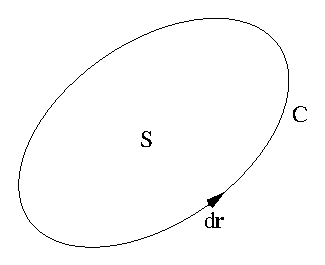
\includegraphics[clip]{1999math-1.eps}
\end{center}

\SubSubQuestion
$\Vec{E}=(x^2-y^2,-2xy)$のとき$\dfrac{\del E_y}{\del x}-\dfrac{\del E_x}{\del y}=0$となることを示し、設問(i)における$\varphi(x,y)$を求めよ。

\SubSubQuestion
点$(x,y)$における接線が、設問(ii)の$\Vec{E}(x,y)$と平行になる曲線群$\varPsi(x,y)=a\quad (a=\text{定数})$を決定せよ。

\end{subsubquestions}

%第2問
\SubQuestion
\begin{subsubquestions}
\SubSubQuestion
行列
\[
\Mat{A} = \begin{pmatrix}
	0 & 1 & 0\\
	1 & 1 & 1\\
	0 & 1 & 0
	\end{pmatrix}
\]
の固有値と固有ベクトルを全て求めよ。ただし、固有ベクトルは正規化せよ。

\SubSubQuestion
\def\root2{\cfrac{1}{\sqrt{2}}}
次の行列
\[
\Mat{X} = \begin{pmatrix}
	\root2 & \root2 & 0\\
	\root2 & -\root2 & 0\\
	0 & 0 & 1
	\end{pmatrix}
\]
により、設問(i)の行列$\Mat{A}$を変換して得られる行列$\Mat{B}=\Mat{XAX^\dagger}$を考える。ただし、$\Mat{X^\dagger}$は$\Mat{X}$のエルミート共役行列である。行列$\Mat{B}$の固有値、固有ベクトルを示せ。ただし、固有ベクトルは正規化せよ。


\SubSubQuestion
エルミート行列$\Mat{A}=(a_{ij})\quad (i,j=1,\ldots,n)$の固有値を$\alpha_i \quad (i=1,\ldots,n)$とする。それらに関して次の2つの量、
\[
F = \sum_{i=1}^n |\alpha_i|^2 \quad,\quad G = \sum_{i,j=1}^n |a_{ij}|^2
\]
を考える。設問(i)の$\Mat{A}$に対して$F$と$G$を求めよ。

\SubSubQuestion
設問(iii)の$F$と$G$の関係を、一般のエルミート行列$\Mat{A}$に対して述べよ。

\end{subsubquestions}

%第3問
\SubQuestion
時刻$t=0$において$x=0$に強さ1の熱を加えたときの、1次元空間におけるその後の熱の伝導は、方程式、
\begin{equation}
\left( \kappa^2 \frac{\del^2}{\del x^2} - \frac{\del}{\del t} \right) G(x,t) = -\delta(x)\delta(t) \qquad \text{($\kappa$は正定数)} \eqname{Q3-1}
\end{equation}
の解$G(x,t)$によって記述される。ただし、$\delta(x)$はディラックのデルタ関数である。また$t=-\infty$で$G(x,t)=0$とする。

\begin{subsubquestions}
\SubSubQuestion
$G(x,t)$のフーリエ変換$g(k,\omega)$を次の式で定義する:
\begin{equation}
G(x,t) = \frac{1}{(2\pi)^2} \int_{-\infty}^{\infty}\int_{-\infty}^{\infty} g(k,\omega)e^{i(kx-\omega t)}\d{k}\d{\omega}\eqname{Q3-2}
\end{equation}
このとき$g(k,\omega)$の満たすべき方程式を式\eqhref{Q3-1}より導き、$g(k,\omega)$を求めよ。

\SubSubQuestion
設問(i)で求めた$g(k,\omega)$を式\eqhref{Q3-2}に代入し、$\omega$積分を実行せよ。

\SubSubQuestion
設問(ii)に続いて$k$積分を実行し、$G(x,t)$を求めよ。ただし、
\begin{equation}
\int_{-\infty}^{\infty} e^{-\alpha^2}\d{\alpha} = \sqrt{\pi}
\end{equation}
を用いてよい。

\end{subsubquestions}

\end{subquestions}
\end{question}
\begin{answer}{教育 数学}{}
\begin{subanswers}
\SubAnswer
\begin{subsubanswers}
\SubSubAnswer
\[ \oint_C (E_x dx + E_y dy) = \iint_S \left(\frac{\partial E_y}{\partial x} - \frac{\partial E_x}{\partial y}\right)dxdy = 0 \]
の時、固定点$O(x_0,y_0)$から$P(x,y)$までの線積分は経路に依らないから
\[ \varphi (x,y) = \int^P_O (E_x dx + E_y dy)  \]
とおける。この場合、線積分が経路に依らないので、まず$x$軸に平行に$(x_0,y_0)\to (x,y_0)$と動かし、次に$y$軸に平行に$(x,y_0)\to (x,y)$と動かす経路を取ると、
\[
\varphi (x,y) = \int_{x_0}^{x} E_x(x,y_0) dx + \int_{y_0}^{y} E_y(x,y) dy
\]
と書くことができる。従って、この式より、
\begin{align*}
\frac{\del \varphi}{\del x} &= E_x(x,y_0) + \int_{y_0}^{y} \frac{\del E_y}{\del x} dy\\
&= E_x(x,y_0) + \int_{y_0}^{y} \frac{\del E_x}{\del y} dy \qquad \left(\because \frac{\del E_y}{\del x}-\frac{\del E_x}{\del y}=0\right)\\
&= E_x(x,y_0) + E(x,y) - E_x(x,y_0)\\
&= E_x(x,y)
\end{align*}
また、
\[
\frac{\del \varphi}{\del y} = E_y(x,y)
\]
が得られる。よって、
\[
\Vec{E} = \Grad \varphi = \left(\frac{\partial \varphi}{\partial x},\frac{\partial \varphi}{\partial y}\right)
\]
と書ける。


\SubSubAnswer
\[ \frac{\partial E_y}{\partial x} = -2y, \quad \frac{\partial E_x}{\partial y} = -2y. \qquad \therefore \frac{\partial E_y}{\partial x} - \frac{\partial E_x}{\partial y} =0 \]
          \begin{align*}
          \varphi (x,y) &= \int^{(x,y)}_O \Vec{E} \cdot {\d{\Vec{r}}} + \varphi(0,0) \\
                        &= \int^{(x,0)}_O E_{x}dx + \int^{(x,y)}_{(x,0)} E_{y}dy + C \quad (Cは定数)\\
                        &= \int^{(x,0)}_{(0,0)} (x^{2} - y^{2}) dx + \int^{(x,y)}_{(x,0)} (-2xy)dy  + C  \\
                        &= \frac{1}{3}x^3 - xy^2 + C
          \end{align*}
          
          
\SubSubAnswer
          $\varPsi (x,y) -a = 0$の法線が$\Vec{E}(x,y)=(x^2-y^2,-2xy)$と直交すれば良い。
          \[ \nabla [\varPsi (x,y) - a] \cdot \Vec{E}(x,y) = 0 \]
          ここで例えば
          \begin{align}
          \frac{\partial \varPsi}{\partial x} &= 2xy \eqname{A1-3}\\
          \frac{\partial \varPsi}{\partial y} &= x^2 - y^2 \eqname{A1-4}
          \end{align}
          を取ることができる。\eqhref{A1-3}より
\[ \varPsi (x,y) = x^2 y + C(y)  (C(y)はyだけの関数)\]
          これを\eqhref{A1-4}に代入して
          \begin{align*}
          x^2 + C^\prime (y) &= x^2 - y^2 \\
                C^\prime (y) &= -y^2 \qquad \therefore C(y) = -\frac{1}{3}y^3 + c (cは定数)
          \end{align*}
\[ \therefore \varPsi (x,y) = x^2 y - \frac{1}{3}y^3 + c \]
          よって求める曲線群は
\[ \varPsi (x,y) = x^2 y - \frac{1}{3}y^3 = a  (aは定数)\]

\end{subsubanswers}


\SubAnswer
\begin{subsubanswers}
\SubSubAnswer
\[\det(\Mat{A} - \lambda \Mat{E}) = \lambda ^2 (1 - \lambda) + 2\lambda 
                         = -\lambda (\lambda - 2)(\lambda + 1) = 0 \] 
  より固有値は$-1,0,2$.\\
  固有値が$-1$の時、長さ$1$の固有ベクトルとして
              $\displaystyle \frac{1}{\sqrt{3}}
              \vect{1}{-1}{1}$,\\
  固有値が$0$の時、長さ$1$の固有ベクトルとして
              $\displaystyle \frac{1}{\sqrt{2}}
              \vect{1}{0}{-1}$,\\

  固有値が$2$の時、長さ$1$の固有ベクトルとして
              $\displaystyle \frac{1}{\sqrt{6}}
              \vect{1}{2}{1}$ 
  がとれる。\\
  よって
	\[
            \frac{1}{\sqrt{3}}
              \vect{1}{-1}{1}
	, \qquad
            \frac{1}{\sqrt{2}}
              \vect{1}{0}{-1}
        , \qquad
            \frac{1}{\sqrt{6}}
              \vect{1}{2}{1}
	\]
  が求める正規化された固有ベクトルである。

\SubSubAnswer
      \begin{align*}
      \Mat{X}\Mat{X}^{\dagger} 
         &=
            \begin{pmatrix}
              \frac{1}{\sqrt{2}} & \frac{1}{\sqrt{2}} & 0 \\
              \frac{1}{\sqrt{2}} & -\frac{1}{\sqrt{2}} & 0 \\
              0 & 0 & 1 
              \end{pmatrix}
            \begin{pmatrix}
              \frac{1}{\sqrt{2}} & \frac{1}{\sqrt{2}} & 0 \\
              \frac{1}{\sqrt{2}} & -\frac{1}{\sqrt{2}} & 0 \\
              0 & 0 & 1 
            \end{pmatrix}\\
         &=
            \begin{pmatrix}
              1 & 0 & 0 \\
              0 & 1 & 0 \\
              0 & 0 & 1 
            \end{pmatrix}
          \end{align*}

      \[
      \therefore \Mat{X}^{\dagger} = \Mat{\Mat{X^{-1}}}
      \]
      
      \textbf{(i)}で求めた各固有ベクトルを
            $\displaystyle
              \Vec{a} \equiv \frac{1}{\sqrt{3}}\vect{1}{-1}{1},\quad
              \Vec{b} \equiv \frac{1}{\sqrt{2}}\vect{1}{0}{-1},\quad
              \Vec{c} \equiv \frac{1}{\sqrt{6}}\vect{1}{2}{1} $
      とおき、$\Mat{P} = (\Vec{a},\Vec{b},\Vec{c})$として行列\Mat{P}を定めると、
      \[
      \Mat{A}\Mat{P} = \Mat{A} (\Vec{a},\Vec{b},\Vec{c}) = (\Vec{a},\Vec{b},\Vec{c})
                \begin{pmatrix}
                -1 & 0 & 0 \\
                0 & 0 & 0 \\
                0 & 0 & 2 
                \end{pmatrix}
         \equiv \Mat{P}\Mat{Q} 
      \]
      となっているので、
	$\Mat{A} = \Mat{P} \Mat{Q} \Mat{P^{-1}}$
      と書ける。
      \begin{align*}
      \Mat{B} = \Mat{X}\Mat{A}\Mat{X^{\dagger}} = \Mat{X}\Mat{A}\Mat{X^{-1}} &= \Mat{X}(\Mat{P}\Mat{Q}\Mat{P^{-1}})\Mat{X^{-1}} \\ &=
 \Mat{X}\Mat{P}\Mat{Q}(\Mat{X}\Mat{P})^{-1}
      \end{align*}
      であるので、
      \[
      \Mat{B}(\Mat{X}\Mat{P}) = \Mat{X}\Mat{P}\Mat{Q}
      \]
      よって
      \begin{align*}
      \Mat{B} (\Mat{X}\Vec{a},\Mat{X}\Vec{b},\Mat{X}\Vec{c}) &=
      (\Mat{X}\Vec{a},\Mat{X}\Vec{b},\Mat{X}\Vec{c})
      \begin{pmatrix}
         -1 & 0 & 0 \\
    	 0 & 0 & 0 \\
         0 & 0 & 2 
      \end{pmatrix}\\
        &= (-1\cdot\Mat{X}\Vec{a},0\cdot\Mat{X}\Vec{b},2\cdot\Mat{X}\Vec{c})
      \end{align*}
      と書けるので、\Mat{B}の固有値は$-1,0,2$であり、$\Mat{X}\Vec{a}、\Mat{X}\Vec{b}、\Mat{X}\Vec{c}$は$\Mat{B}$の固有ベクトルとなっている。また
      \begin{align*}
      (\Mat{X}\Vec{a},\Mat{X}\Vec{a}) &= (\Vec{a},\Mat{X^{\dagger}}\Mat{X}\Vec{a}) \\
                                &= (\Vec{a},\Vec{a})   (\because \Mat{X^{\dagger}}\Mat{X} = \Mat{E}) \\
                                &= 1     (\because\Vec{a}は単位ベクトル)
      \end{align*}
      よって$\Mat{X}\Vec{a}$は単位ベクトルであることが言える。\\
      以上より、$\Mat{X}\Vec{a}、\Mat{X}\Vec{b}、\Mat{X}\Vec{c}$は$\Mat{B}$の正規化された固有ベクトルであることが言える。よって求めるベクトルは、
      \[
      \Mat{X}\Vec{a} = \frac{1}{\sqrt{3}} \vect{0}{\sqrt{2}}{1} ,\qquad
      \Mat{X}\Vec{b} = \frac{1}{2} \vect{-1}{1}{-\sqrt{2}} ,\qquad
      \Mat{X}\Vec{c} = \frac{1}{2\sqrt{3}} \vect{3}{-1}{\sqrt{2}}
      \]
      
      
\SubSubAnswer
      \begin{gather*}
      F = \sum_{i=1}^{3} |\alpha_i | = |-1|^2 + |0|^2 + |2|^2 = 5\\
      G = \sum^{3}_{i,j=1} |a_{ij}|^2 = 5
      \end{gather*}
      
\SubSubAnswer
\[
\Mat{B} = (b_{ij}) \equiv
\left(
\begin{array}{@{\,}ccccc@{\,}}
   \alpha_1 & 0 & 0 & \ldots & 0 \\
   0 & \alpha_2 & 0 & \ldots & 0 \\
   0 & 0 & \alpha_3 & \ldots & 0 \\
   \vdots & \vdots & \vdots & \ddots & \vdots \\
   0 & 0 & 0 & \ldots & \alpha_n
\end{array}
\right)
\]
とおく。

エルミート行列$\Mat{A}$はユニタリ行列$\Mat{U}$を用いて、
\[
\Mat{U^\dagger A U} = \Mat{B}
\]
のように対角化できる。

まず、
\begin{equation}
\sum_{i,j=1}^n |b_{ij}|^2 = \sum_{i=1}^n |\alpha_i|^2 = F \eqname{F}
\end{equation}
が成り立つ。

以下では、和記号を明記しない場合を除いては、同じ添字が2度現れたときには和を取るものとすると、
\begin{align}
\sum_{i,j=1}^n |b_{ij}|^2 &= \sum_{i,j=1}^n |(\Mat{U^\dagger A U})_{ij}|^2 \nonumber\\
&= (\Mat{U^\dagger A U})_{ij}\overline{(\Mat{U^\dagger A U})}_{ij} \nonumber\\
&= \left(U_{ik}^{-1}a_{kl}U_{lj}\right)\left(U_{mi}\overline{a}_{mn}U_{jn}^{-1}\right) \nonumber\\
&= \delta_{mk}\delta_{ln}a_{kl}\overline{a}_{mn} \nonumber\\
&= a_{kl}\overline{a}_{kl} \nonumber\\
&= G \eqname{G}
\end{align}

ここで、ユニタリ行列に関する次の性質を用いた。
\begin{align*}
\Mat{U}^\dagger &= \Mat{U}^{-1}\\
\overline{\Mat{U}}^\dagger &= \Trans{\Mat{U}}\\
\overline{\Mat{U}} &= \Trans{\left(\Mat{U}^{-1}\right)\!\!}
\end{align*}

\eqhref{F}\eqhref{G}より、
\[
F = G
\]
が成り立つ。



      
\end{subsubanswers}

\SubAnswer
\begin{subsubanswers}
      \SubSubAnswer
      \eqhref{Q3-2}式と
      \[
      \delta (x)\delta (t) = \frac{1}{(2 \pi)^2}\int^{\infty}_{-\infty}dk\int^{\infty}_{-\infty}d\omega \ e^{i(kx-\omega t)}
      \]
      を\eqhref{Q3-1}式に代入すると、
      \[
      \int^{\infty}_{-\infty}dk\int^{\infty}_{-\infty}d\omega (-\kappa^2 k^2 + i\omega) g(k,\omega)e^{i(kx-\omega t)} = - \int^{\infty}_{-\infty}dk\int^{\infty}_{-\infty}d\omega e^{i(kx-\omega t)}
      \]
      従って、$g(k,\omega)$の満たすべき方程式は、
      \[
      (\kappa^2 k^2 - i\omega) g(k,\omega) = 1
      \]
      従って、
      \[
       g(k,\omega) = \frac{1}{\kappa^2 k^2 - i\omega}
      \]
      である。
      
      
\SubSubAnswer
      
      \textbf{(i)}で求めた$g(k,\omega)$を\eqhref{Q3-2}に代入すると、
      \[
      G(x,t) = \frac{1}{(2 \pi)^2}\int^{\infty}_{-\infty}dk\int^{\infty}_{-\infty}d\omega \frac{1}{\kappa^2 k^2 - i\omega} e^{i(kx-\omega t)}
      \]
      これを$\omega$について積分する。今、
      \[
      I=\frac{1}{2 \pi}\int^{\infty}_{-\infty}d\omega \frac{e^{-i\omega t}}{\kappa^2 k^2 - i\omega}
      \]
      なる$I$を考えるとする。$z=\kappa^2 k^2 - i\omega$とおくと、
      \[
      \begin{cases}
         \displaystyle I = \frac{i}{2 \pi} \int^{r-i\infty}_{r+i\infty}\!dz\ \frac{e^{zt}}{z}e^{-\kappa^2 k^2 t} \\
         r = \kappa^2 k^2
      \end{cases}
      \]
      となる。さて、ステップ関数$\theta (t)$は、
      \[
      \theta (t) = \frac{1}{2\pi i}\int^{R+i\infty}_{R-i\infty}\!dz\ \frac{e^{zt}}{z}=
      \begin{cases}
       1 (t>0) \\
       0 (t<0)   (Rは任意の実数)
       \end{cases}
      \]
      ということが、留数定理から分かる。従って$I$は、
      \[
      I = \theta (t) e^{-\kappa^2 k^2 t}
      \]
      である。従って、
      \[
      G(x,t) = \frac{1}{2\pi}\int^{\infty}_{-\infty}\!dk\ \theta (t)e^{-\kappa^2 k^2 t}e^{ikx}
      \]
      
\SubSubAnswer
      設問\textbf{(ii)}の結果より
\begin{align*}
      G(x,t) &= \frac{1}{2\pi} \theta (t) \int^{\infty}_{-\infty}dk\ \exp\left[-\kappa^2 t\left(k-\frac{ix}{2\kappa^2 t}\right)^2\right] \exp\left(-\frac{x^2}{4\kappa^2 t}\right) \\
             &= \frac{1}{2\pi} \theta (t) \sqrt{\frac{\pi}{\kappa^2 t}} \exp\left(-\frac{x^2}{4\kappa^2 t}\right)
\end{align*}
      
\end{subsubanswers}
    
\end{subanswers}
\end{answer}



\end{document}

